\chapter{Background}
\section{Cothority}

\paragraph{}
The Cothority framework is composed of multiple protocols, services, and apps. At its current stage of development, CPMAC only supports the CISC and PoP apps, but it is intended to progressively feature and integrate more apps. We now present these two apps in more depth.

\subsection{CISC}

// TODO: INSERT

\subsection{PoP}

\paragraph{}
The PoP app of the cothority framework is used to generate and verify proof of personhood, which indicates that a user is a human being. Personhood is proven through stating that a specific person was at a precise location at a particular time and thus that this user is not a bot or any other kind of human-simulating program. Before continuing, we define some important terms.

\begin{description}[style=nextline]
\item[Key Pair] In cryptography a key pair is composed of a public and private key, the public key is shared with anyone as opposed to the private key which has to remain secret to the owner of the key pair. Typically a message is encrypted and/or signed with the private key and can then be decrypted and/or verified with the public key.

\item[Conode Linking] Before being able to exchange data with a cothority node, one has to link itself to it, this is done by registering the public key on the conode after having shown that one has access to it (typically by reading a short PIN in the server logs).

\item[PoP Party] A PoP party is a gathering of people wanting to prove that they are human beings by showing everyone that they are able to come to a specific location at a specific time.

\item[Organizer (Org)] An organizer is someone hosting a PoP party by providing a conode. Since there are multiple organizers, their conodes form a cothority network and thus host the party in a distributed and decentralized manner.

\item[Attendee (Att)] An attendee is someone present at a PoP party without providing a conode and thus only attending it for the sake of a PoP token (an organizer can at the same time be an attendee).

\item[PoP Party Configuration/Description (Config/Desc)] The configuration or description of a PoP party defines all the required properties. It should include the name, the date and time, the location and a list of all the hosting conodes (which is commonly refered to as a roster) for the PoP party.

\item[Attendee Registration] The attendee registration is the process of registering all the public keys of the attendees on each of the organizers conodes, all the organizers have to do it separately for their own server.

\item[Final Statement] A final statement of a PoP party is generated by the cothority network composed of the hosting conodes, it is composed of a PoP party configuration, all the public keys of the attendees, the collective signature generated by the hosting conodes and a boolean to state if this PoP party has been merged with another one.

\item[PoP Token] A PoP token is the final token proving that the holder is a human being and attended this particular PoP party, it is composed of a final statement and a key pair.
\end{description}

\paragraph{}
First, all of the party organisers must agree on a date, time, and location. Once these specifications are set, all of the attendees (including the organisers) meet at the right location, date, and time. Each organiser has to link with a conode, complete the PoP configuration, and register it on his or her own conode; the organisers then receive the identification of this PoP party, which is henceforth used as a reference to uniquely identify it. Once every organiser registered the configuration and the PoP party is over, each one registers the list of all of the public keys of the attendees. During this step, the organisers have to ensure that each attendee has registered one and only one public key; this is a crucial step because otherwise an attendee could generate PoP tokens for every public key that he or she registered. This would then contradict the important criterion that each human being is unique and thus should only receive one PoP token for each attended party. Once every organiser registered all of the attendees, the cothority composed of their conodes finalises the party by generating the final statement containing all relevant information, which includes a collective signature. This final statement is then sent to the attendees so that they can generate their PoP token by linking this final statement to their key pair.

\section{Technologies}

\paragraph{}
Throughout this project many different technologies were used, we are now quickly presenting the main ones in a few words.

\subsection[Elliptic Curve Cryptography]{Elliptic Curve Cryptography\raisebox{.3\baselineskip}{\normalsize\footnotemark}}
\footnotetext{\url{https://en.wikipedia.org/wiki/Elliptic-curve_cryptography}}

\paragraph{}
This public-key cryptographic system using elliptic curves (EC) has been independently suggested by Neal Koblitz and Victor S. Miller in 1985. EC algorithms only entered wide use in 2004 to 2005. The major difference with prior cryptographic protocols (for example DSA or RSA), that were defined over multiplicative groups of finite fields, is that EC cryptography uses point addition instead of modular exponentiation. This results in faster computation.

\subsection[Schnorr Signature]{Schnorr Signature\raisebox{.3\baselineskip}{\normalsize\footnotemark}}
\footnotetext{\url{https://en.wikipedia.org/wiki/Schnorr_signature}}

\paragraph{}
The schnorr signature algorithm is considered as one of the simplest scheme being provably secure in a random oracle model to produce digital signatures. In addition to that, the schnorr algorithm is efficient and produces short signatures.

\subsection[Protocol Buffers]{Protocol Buffers\raisebox{.3\baselineskip}{\normalsize\footnotemark}}
\footnotetext{\url{https://en.wikipedia.org/wiki/Protocol_Buffers}}

\paragraph{}
Developed by Google, this data interchange format is a language- and platform-neutral structured data serializer. Protobuf allows to define data structures once and then easily write to or read from data streams. In this particular project it is used to encode JS objects and decode byte streams received from the conodes and thus ease the process of data exchange.

\subsection[Websocket]{Websocket\raisebox{.3\baselineskip}{\normalsize\footnotemark}}
\footnotetext{\url{https://en.wikipedia.org/wiki/WebSocket}}

\paragraph{}
This communication protocol uses a single TCP connection to send data back and forth while keeping the connection open, thus facilitates real-time data transfers from and to the server. It is the used protocol for data exchange with the conodes.

\begin{figure}[h]
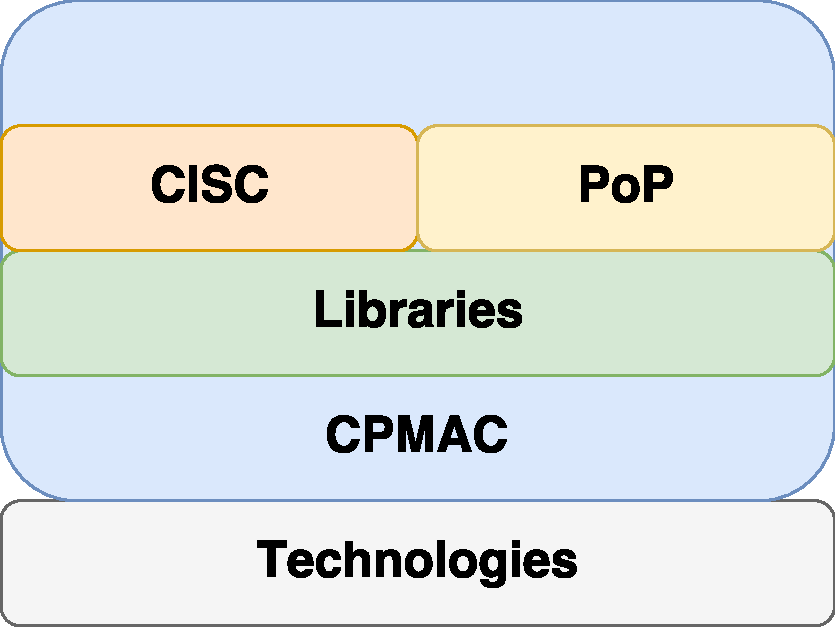
\includegraphics[scale=.5]{graphic/cpmac.pdf}
\centering
\caption{CPMAC Structure}
\end{figure}
